\documentclass[12pt]{article}

\usepackage[backend=biber,style=mla]{biblatex}
\usepackage[margin=.7in]{geometry}
\usepackage[utf8]{inputenc}
\usepackage{setspace}
\usepackage{amsmath}
\usepackage{amssymb}
\usepackage{mathtools}
\usepackage{esint}
\usepackage{titlesec}
\usepackage{graphicx}
\usepackage{wrapfig}
\usepackage{blindtext}
\usepackage{fancyhdr}
\usepackage{multicol}

\addbibresource{/home/krttd/documents/UAH.bib}

\pagestyle{fancy}
\lhead{}
\chead{}
\cfoot{}
\rhead{Dodson \thepage}

\renewcommand*{\bibfont}{\normalsize}

\titleformat{\section}
{\large}{}{0em}{}[\titlerule]

\begin{document}
\thispagestyle{empty}

\begin{center}\LARGE
How to publish to the SPoRT Blog
\end{center}

\begin{center}\large
  By: Mitchell Dodson
\end{center}

\begin{multicols}{2}

{
  \centering
  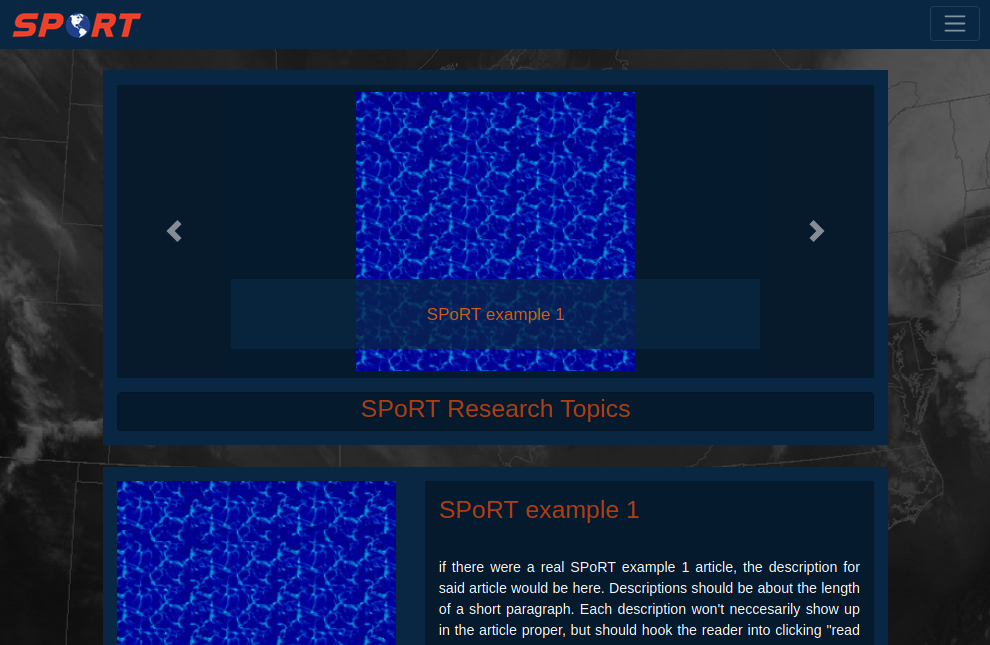
\includegraphics[width=.95\linewidth]{./figures/website-ss.png}
}

\section{What is the SPoRT blog?}

The SPoRT blog is a utility open to all SPoRT civil servants, contractors, and graduate students which allows you to quickly publish summaries of your research to the public, organize outreach events, and spotlight groups and individuals for their exceptional work. The blog is hosted locally on the Weather web server, which gives you the ability to publish to the blog from any machine in the local network. Please contact Paul Meyer for more information on how to be authorized to publish. The blog site was developed by SPoRT undergraduates Mitchell Dodson and Ben Houser under the supervision of Paul Meyer and Roger Allen.

\section{Command-Line Interface}

Blog articles must be published from a machine on the SPoRT network, which means graphical interfaces are unfortunately not a possibility. In order to make publishing as simple as possible, the development team designed a strightforward command-line interface (CLI) to take care of the process. When you SSH into a SPoRT machine, the publishing software will be availiable in the form of the commands \texttt{blogprepare} and \texttt{blogpublish}, along with several options. Currently, docx, html, and rtf formats are supported.

\vfill\null
\columnbreak

\section{Publishing steps}
\begin{enumerate}
  \item{If your article is currently stored on your machine, copy the article document to the remote SPoRT machine that you want to publish from.}
  \item{ssh into the remote SPoRT machine and change your directory to the same one as the article.}
  \item{run \texttt{\$blogprepare ./the-article.docx} along with any other options found in Section \ref{cli}. It is recommended that you at least specify a thumbnail image with \texttt{-i}.}
  \item{Optionally fill out the module.json form that the script has placed in your current directory. If you don't do this, a title and description will be selected automatically.}
  \item{run \texttt{\$blogpublish ./module.json} on the json document in order to finish the publishing process.}
\end{enumerate}

\section{CLI Options}
\label{cli}

The following options can be passed to either \texttt{blogprepare} or \texttt{blogpublish}. Provide the arguments in any order you like as, long as the image path always immediately follows the \texttt{-i} flag.

\noindent
\texttt{--keep-article}: save the original article and thumbnail image to the current machine.

\noindent
\texttt{--keep-module-json}: keep the json form for setting title/description.

\noindent
\texttt{-i} \textit{/path/to/image}: specify the path to the article thumbnail image. If the image is not a 1x1 aspect ratio, it will be automatically cropped.

\section{Editing articles after publishing}

If you would like to make a change to an article that has already been uploaded to the blog site, please contact Mitchell Dodson (\textit{email@address}) or Paul meyer (\textit{email@address})

\end{multicols}
\printbibliography
\end{document}
